\chapter{Manual de Operação}\label{cap_3_Metodologia}

Quando o hardware é sintetizado na FPGA, um contador decresecente até 0, começando do 9, se inicia, como pode ser visto na Figura \ref{fig:3.1}.

%Foto da fpga quando o contador está no 0
\begin{figure}[H]
	\centering
	\includegraphics[width=1\columnwidth]{FIGURAS/cap_3/placa9.jpg}
	\caption{Início do contador decrescente de 10 segundos.}
        \label{fig:3.1}
\end{figure}

Quando esse contador começa, o usuário tem dez segundos para inserir uma senha nos push-buttons, que podem ser vistos na Figura \ref{fig:3.2}. 

%Mesma foto da 21, mas aqui dando destaque aos push-buttons
\begin{figure}[H]
	\centering
	\includegraphics[width=1\columnwidth]{FIGURAS/cap_3/localpb.png}
	\caption{Local em que se inserem as senhas.}
        \label{fig:3.2}
\end{figure}

Cada push-button ativa um LED, como pode ser visto nas Figuras \ref{fig:3.3}, \ref{fig:3.4}, \ref{fig:3.5} e \ref{fig:3.6}.

%Figura com o primeiro push-button(1) e o seu LED acesso
\begin{figure}[H]
	\centering
	\includegraphics[width=1\columnwidth]{FIGURAS/cap_3/pb1.png}
	\caption{Push-button de menor significância com o seu LED acionado.}
        \label{fig:3.3}
\end{figure}

%Figura com o segundo push-button significativo acionado e seu LED acesso
\begin{figure}[H]
	\centering
	\includegraphics[width=1\columnwidth]{FIGURAS/cap_3/pb2.png}
	\caption{Push-button de segunda menor significância com o seu LED acionado.}
        \label{fig:3.4}
\end{figure}

%Figura com o 3 push-button acionado e seu LED acesso
\begin{figure}[H]
	\centering
	\includegraphics[width=1\columnwidth]{FIGURAS/cap_3/pb3.png}
	\caption{Push-button de terceira menor significância com o seu LED acionado.}
        \label{fig:3.5}
\end{figure}

%Figura com o push button de maior significância ativado e seu LED acesso
\begin{figure}[H]
	\centering
	\includegraphics[width=1\columnwidth]{FIGURAS/cap_3/pb4.png}
	\caption{Push-button de maior significância com o seu LED acionado.}
        \label{fig:3.6}
\end{figure}


Cada vez que o usuário precionar um push-button, um buzzer, com uma devida frequência irá ser acionado. 

Após os 10 segundos, ou seja, quando o contador chega a 0, como mostrado na Figura \ref{fig:3.7}, se a senha inserida for a correta, um devido buzzer será acionado, o contador voltará a 9, como mostrado na Figura \ref{fig:3.1}, e o usuário terá mais 10 segundos para inserir uma outra senha. Mas, se a senha inserida for a incorreta, um outro buzzer será acionado, o contador voltará a 9 e o usuário terá que inserir a primeira senha novamente.

\begin{figure}[H]
	\centering
	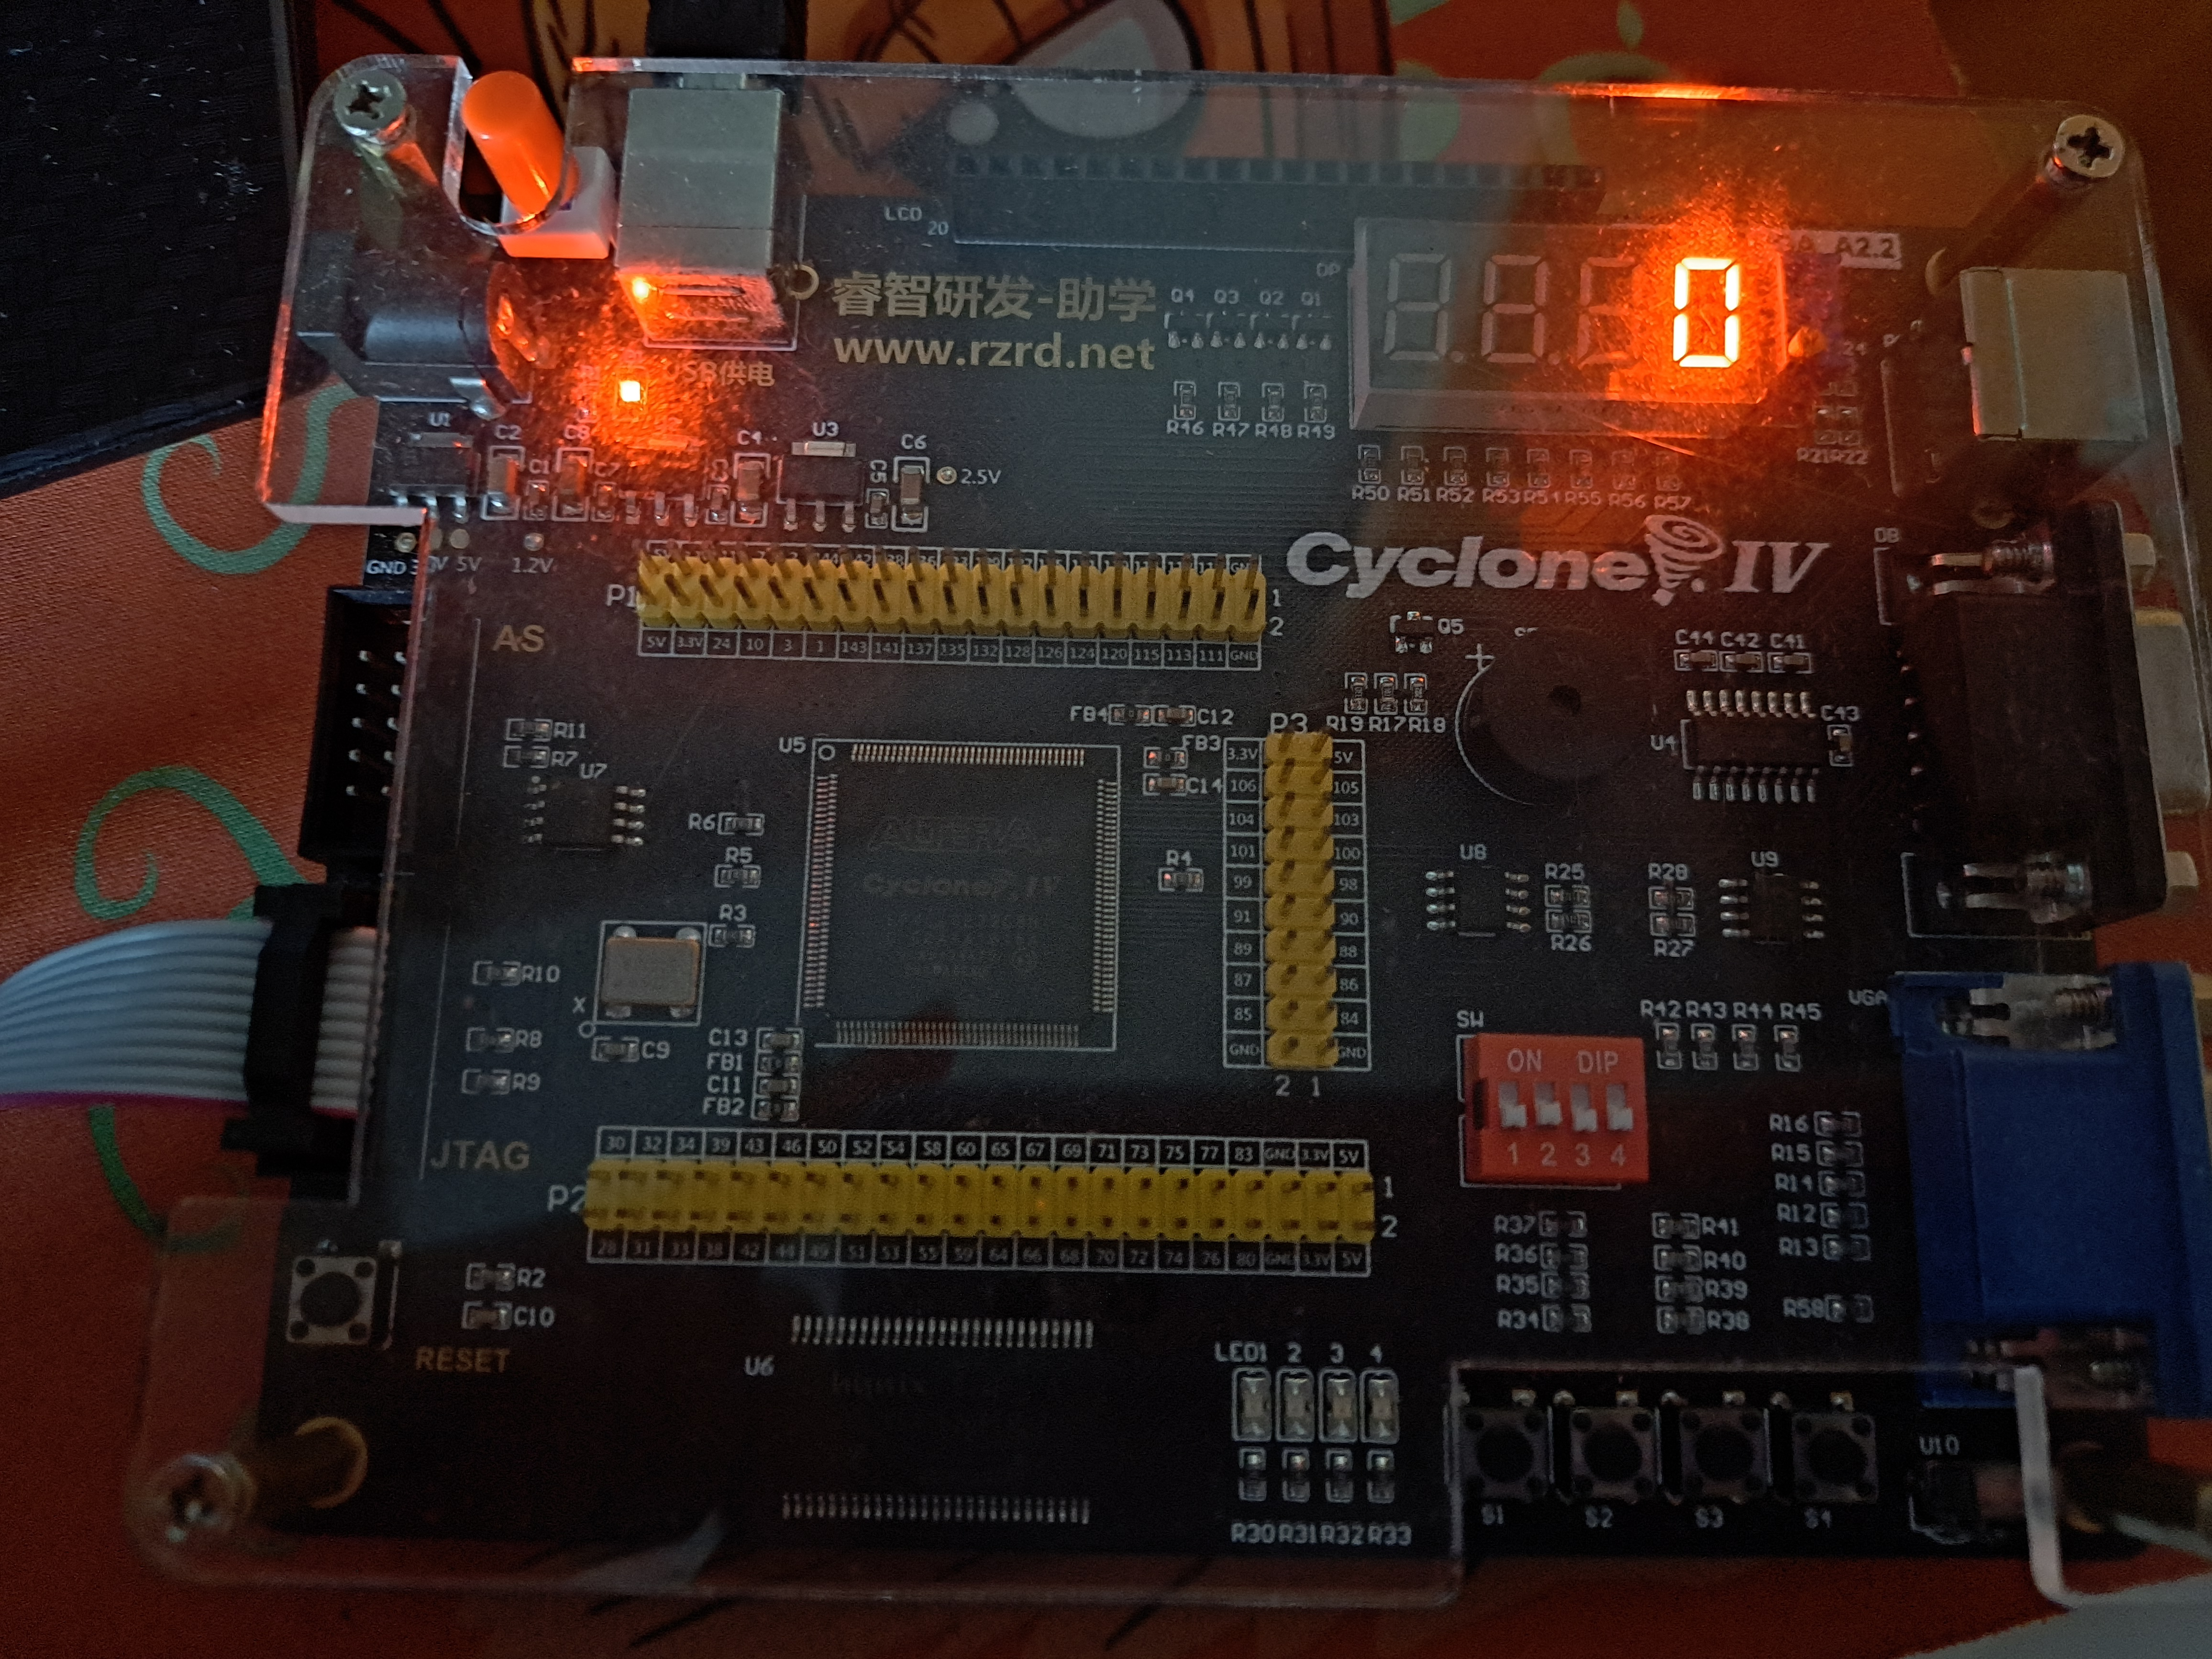
\includegraphics[width=1\columnwidth]{FIGURAS/cap_3/placa0.jpg}
	\caption{Fim do contador decrescente de 10 segundos}
        \label{fig:3.7}
\end{figure}

No total são 16 hexadecimais que precisam ser inseridos e, para cada uma deles, o usuário terá 10 segundos para inseri-los. Toda vez que o usuário errar uma senha, o hardware é reiniciado. Se o usuário inserir o décimo sexto hexadecimal e um buzzer for ativado indefinidamente, isso significa que o usuário acertou todas as 16 senhas. 

